\documentclass[12pt]{report}
\usepackage[utf8]{inputenc}
\usepackage{graphicx}
\usepackage[english]{babel}
\graphicspath{ {D:/licenta/sounds/paper/images/} }
\usepackage[nottoc,notlot,notlof]{tocbibind}
\usepackage{setspace}
\usepackage{subcaption}
\usepackage[table,xcdraw]{xcolor}
\usepackage[normalem]{ulem}
\usepackage[paper=a4paper,margin=1in]{geometry}

\begin{document}

\title{%
  { \huge Babeș-Bolyai University\\
  Faculty of Mathematics and Computer\\
  Science\\
  Computer Science English Specialisation}
\ \\
  \ \\
  {\huge Diploma Thesis}
  \ \\
  \ \\
  \ \\
  High freqeuncy audio steganography\\
  Practical application \\
    and comparisons with other techniques
  \ \\
  \ \\
  \ \\
  \ \\
  {%
    \begin{flushleft}%
       Dr. Lecturer Crivei Septimiu
      \end{flushleft}}
      {%
  \begin{flushright}
      Paius Teodor-Marian
  \end{flushright} }}

\maketitle



\newgeometry{top=1in,bottom=1in,right=1.5in,left=1.5in}

\setstretch{1.5}

\begin{abstract}
Steganography is the practice of concealing a file, message, image, or video within another file, message, image, or video. This paper focuses on the domain of digital signal processing and audio concealment of messages. Apart from other common environments such as images or plain text, sound also represents a good way of transmitting hidden messages. The techniques present in this thesis can be applied not only to the target range of human hearing but can also be implemented with some degree of resemblance to other domains of higher frequencies (radio waves or electromagnetic waves).
\end{abstract}

\tableofcontents


\chapter{Introduction}
\section{Motivation}
Apart from being a chance to delve deeper into a domain of computer science where I had less experience previously, this work was also developed with the idea of improving existent security systems in mind. The sounds and how computers "recognize" them present on one had an interesting challenge to make effective use of them to hide messages and on the other hand a good way of combining the robustness of mathematical methods with the huge processing power of today's computers.
\section{Context}
Today we live in a world where data confidentiality is of utmost importance. While the techniques of cryptography offer far more security potential than plain steganography, the existence of encrypted messages is obvious for an attacker, so attacks are inevitable. A good practice would be to hide this message, being them encrypted or not. Here is where steganography could have an impact. As symmetric key cryptography, the strength of a technique lies in a secret known to both parties that take part in communication. Of course, some steganographic techniques have weaker hiding systems ( Least significant byte method ) than others ( phase coding or high-frequency encoding ). By hiding the message, it wouldn't present an immediate chance for an attacker as file such images or audio are sent over the internet with millions each hour.
\section{Objective}
The objective of this work is to study in more detail an area of the art of steganography which is not as frequently used as it should be, and to create an effective way of hiding messages in sound in such a manner that only the sender and the receiver of the message could know to decode. The paper proposes a method which has different variable parameters that can be sent in advance between the participants of the conversation using similar techniques like the know key exchange methods used in everyday cryptography systems such as AES or DES/3DES.

The aim of this project is by no means to replace the existing cryptographic methods used in data obfuscation. On the contrary, I consider that they could be used together with this steganographic method to mitigate the possible DOS attacks over an encrypted message those being now hidden inside a carrier object.
\section{Structure}
This project consists of a theoretical overview of the current steganographic techniques and the description of an algorithm which makes use of high-frequency noise to hide certain messages, together with a practical application developed in Python to support the claims made in this report. 



\chapter{Theoretical background}

The commonly stated range of human hearing is 20 Hz to 20 kHz. Under ideal laboratory conditions, humans can hear sounds as low as 12 Hz and as high as 28 kHz, though the threshold increases sharply at 15 kHz in adults, corresponding to the last auditory channel of the cochlea. Humans are most sensitive to (i.e., able to discern at lowest intensity) frequencies between 2,000 and 5,000 Hz. Based on this a right way of hiding information is exploiting this human weakness and encoding particular messages in audio files disguised as short sequences of high-frequency signals.




\section{Overview of steganography}
The word steganography comes from the Greek language being derived from the two Greek words \emph{steganos}(covered) and \emph{graphein}(to write) referring to the art of enabling communication that uses methods of hiding information in plain sight. In the field of computer science, steganography is the practice of concealing a file, message, image, or video within another file, message, image, or video.
The advantage of steganography over cryptography alone is that the intended secret message does not attract attention to itself as an object of scrutiny. Plainly visible encrypted messages, no matter how unbreakable they are, arouse interest and may in themselves be incriminating in countries in which encryption is illegal.\cite{note4}

\begin{figure}[!h]
\centering
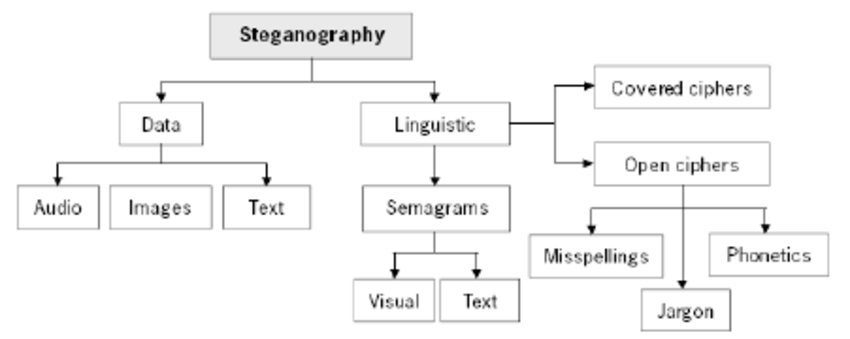
\includegraphics[width=1\textwidth]{steganography}
\caption{General classification of steganographic methods}
\label{fig:steganography}
\end{figure}

The process of detecting specific messages hidden inside a stego-object (image, sound, video) is called steganalysis. The goal of steganalysis is to identify suspected packages, determine whether or not they have a payload encoded into them, and, if possible, recover that payload. 
Unlike cryptanalysis, in which intercepted data contains a message (though that message is encrypted), steganalysis generally starts with a pile of suspect data files, but little information about which of the files, if any, contain a payload. The steganalyst is usually something of a forensic statistician and must start by reducing this set of data files (which is often quite large; in many cases, it may be the entire set of files on a computer) to the subset most likely to have been altered.

Usual methods of steganalysis consist of structural detection - the difference in file properties(size, checksum, headers) or statistical detection - changes in patterns of bits, LSB changes or histogram analysis.

The algorithm proposed in this paper is designed to reduce the efficiency of such methods and to limit the possibility of detection caused by noticeable changes in file structure, composition, or the appearance of anomalies in the stego-object.

\section{Overview of digital signal processing}
\subsection{Sound}
In physics, the sound is a vibration transmitted through different environments: solid, gas, or liquids. Sound can be divided mostly into two parts: pressure and time. These two are the characteristics present in every wave, and because of this, a sound can be considered a continuous signal. The human ear, through its mechanisms, "catches" this stimulus and converts it in electrical signals which are sent to the brain to be analyzed. This process is not perfect, and this is the key fact on which this method relies.

Although there are many complexities regarding sound transmission, most of the time, sound can be characterized by the following properties:
\begin{itemize}
    \item Frequency
    \item Amplitude
    \item Speed of sound
    \item Direction
\end{itemize}
In this method, we are interested just in the first two properties: frequency and amplitude.

\subsection{DSP(Digital sound processing)}
To be able to analyze an analog(continuous) signal in a digital environment, it must first be converted using an analog-to-digital converter. This process is composed of 2 major stages: discretization and quantization. This would transform a continuous signal in a set of consecutive frames equidistant in time, and characterized by a certain amplitude. This representation is also known as time domain. It is used to visualize better the overall image of a sound described as a wave. In (fig \ref{fig:samp_rate}) we can observe the discretization of a sinusoidal wave.

\begin{figure}
\centering
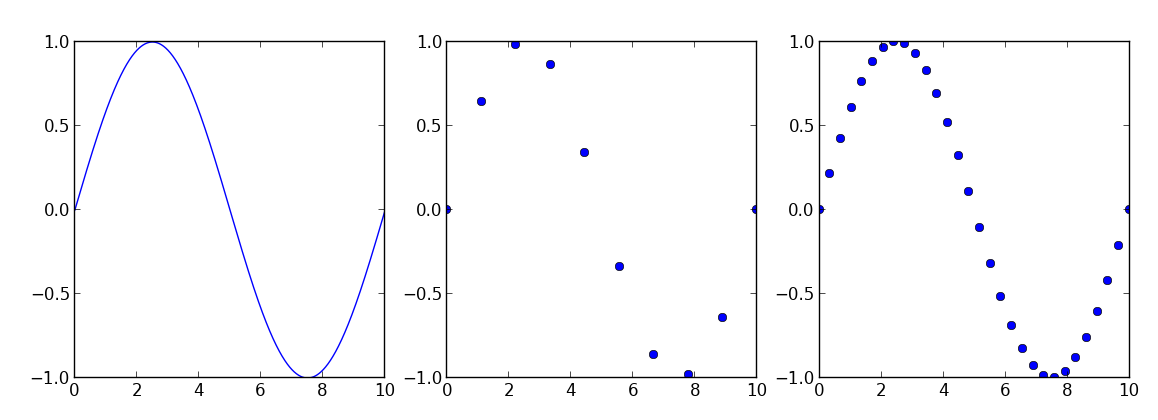
\includegraphics[width=1\textwidth]{sampling_rate}
\caption{Continous signal splitted in discrete samples}
\label{fig:samp_rate}
\end{figure}

Another domain that is of vital importance to us is the frequency domain. Usually, to change the time domain into the frequency domain, a Fourier transform is applied over the discrete samples of the sound. This process converts the time domain samples into frequencies and amplitudes (fig \ref{fig:fourier}).

\begin{center}
\begin{math}
F\left(\zeta \right)\:=\:\int _{-\infty }^{\infty }\:f\left(x\right)e^{-2\pi x\zeta }dx
\end{math}
\end{center}

When the independent variable x represents time, the transform variable represents frequency (e.g., if time is measured in seconds, then then the frequency is in hertz). Under suitable conditions, f is determined via the inverse transform: 
\begin{center}
\begin{math}
F\left(\zeta \right)\:=\:\int _{-\infty }^{\infty }\:f\left(x\right)e^{-2\pi x\zeta } d\zeta
\end{math}
\end{center}
\begin{figure}[!h]
\centering
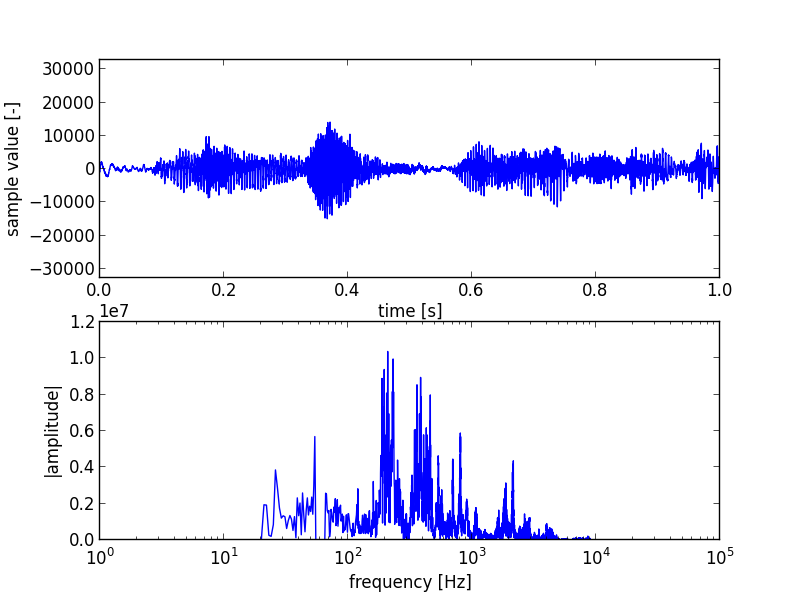
\includegraphics[width=1\textwidth]{fourier}
\caption{Fourier transform applied over a sound}
\label{fig:fourier}
\end{figure}
This way a sound can be reconstructed exactly by reversing the transformation, mainly using the Fourier inverse transform, to change a set of frequencies to the original sound from with they appeared. Also, any change performed over the frequency domain carries on to the time domain. Using serval techniques such as low pass filter or highpass filter, certain ranges of frequencies could be attenuated, this being used mainly to smooth the sound and to clear any noise that could appear during transmission.





The \emph{Nyquist–Shannon} sampling theorem states that a signal can be accurately reconstructed from its samples if the sampling frequency is greater than twice the highest frequency component in the signal. In practice, the sampling frequency is often significantly higher than twice the Nyquist frequency\cite{note5}. In this case, where the target range is about 20-26 kHz, a sampling rate of 48000 samples/second is almost at the limit, meaning that some higher frequencies might be omitted and loss of accuracy, so a higher sampling rate was chosen: 96000 samples/second.


\section{Just a little bit of anatomy}
A primary measure of hearing is afforded by an audiogram (fig \ref{fig:human_hearing}), a graph of the absolute threshold of hearing (minimum discernible sound level) at various frequencies throughout an organism's nominal hearing range. The commonly stated range of human hearing is 20 Hz to 20 kHz.Under ideal laboratory conditions, humans can hear a sound as low as 12 Hz and as high as 28 kHz, though the threshold increases sharply at 15 kHz in adults. Humans are most sensitive to (i.e., able to discern at lowest intensity) frequencies between 2,000 and 5,000 Hz. Individual hearing range varies according to the general condition of a human's ears and nervous system. The range shrinks during life, usually beginning at around the age of eight with the upper-frequency limit being reduced. Women typically experience a lesser degree of hearing loss than men, with a later onset. Men have approximately 5 to 10 dB greater loss in the upper frequencies by age 40\cite{note6}.

\begin{figure}[h]
\centering
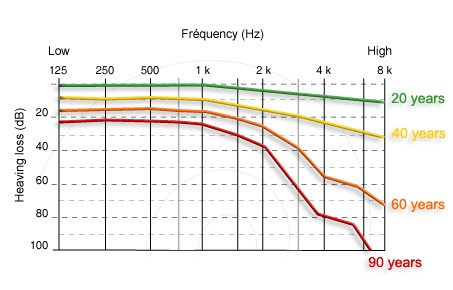
\includegraphics[width=1\textwidth]{human_hearing}
\caption{Human hearing audiograms based on age\cite{note7} MUST CHANGE BAD!!}
\label{fig:human_hearing}
\end{figure}

This practical application of this work focuses on the range of 15-24 kHz with a variable sound amplitude as a program doesn't need a very high signal amplitude to recognize it. Preferably the lower end of the encoding range should be as high as possible to exclude the possibility of individual humans hearing the noise added, but due to hardware limitations, this threshold shouldn't pass 24-25 kHz (to be further discussed in this paper).


As the range of human hearing is variable from one person to another, there exists the possibility of some persons hearing certain anomalies at the lower end of the frequency specter used in this method, but the application features a mechanism to prevent such detections by raising the overall height of the frequencies used.

\chapter{The application}
For proving the concept of hiding information using high-frequency signals, a Python application was implemented
\section{Chosen approach}
The general method consists of several modules, each specialized in specific tasks. The aim of the application is to generate sinusoidal wave noise and to insert it inside a carrier file, and after that to be able to extract the information using the Fourier transform applied on well defined segments of the sound to get the data from the time domain to the frequency domain where it can be analyzed to find if it contains hidden data. By repeating this process on the entire file, the message could be recreated with accuracy as long as the sound hasn't been corrupted in the meantime with other high-frequency noises.


\begin{figure}[h!]
\centering
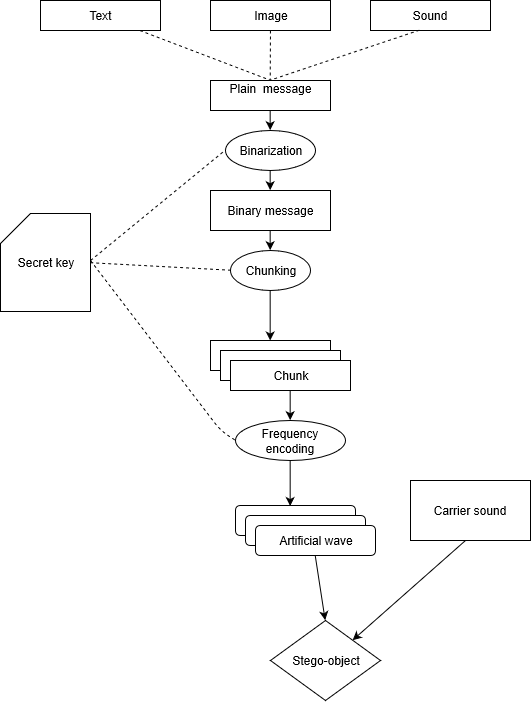
\includegraphics[width=1\textwidth]{flow}
\caption{General flow of the method}
\label{fig:flow}
\end{figure}

\section{Design}
Initially, the work for this project consisted of several prototypes. As I had no previous knowledge in signal processing during this phase, I compared my results to visualizations created in Audacity. After that followed the initial development of a console application which modifies in place a certain sound to hide a constant wave of a certain frequency. To make the application more accessible, I resolved to use the visual library for python Tkinter with its integration of Matlab plotting. One cornerstone of the development was the ability to send the modified sound through whatever channel of communication from one device to another and to be able to recognize the modified frequencies. One first attempt was to send it through the air, from the speakers to a microphone. However, this approach did not prove to be successful, as a lot of the sounds properties were lost during transportation. As I didn't want to digitally copy the sound and then paste it using USB connection as it didn't prove anything regarding the usefulness of this approach, the only other alternative was to send it through audio ports. This way, the sound was sent from one soundcard to the other; the loss is minimal.

\begin{figure}[h]
\centering
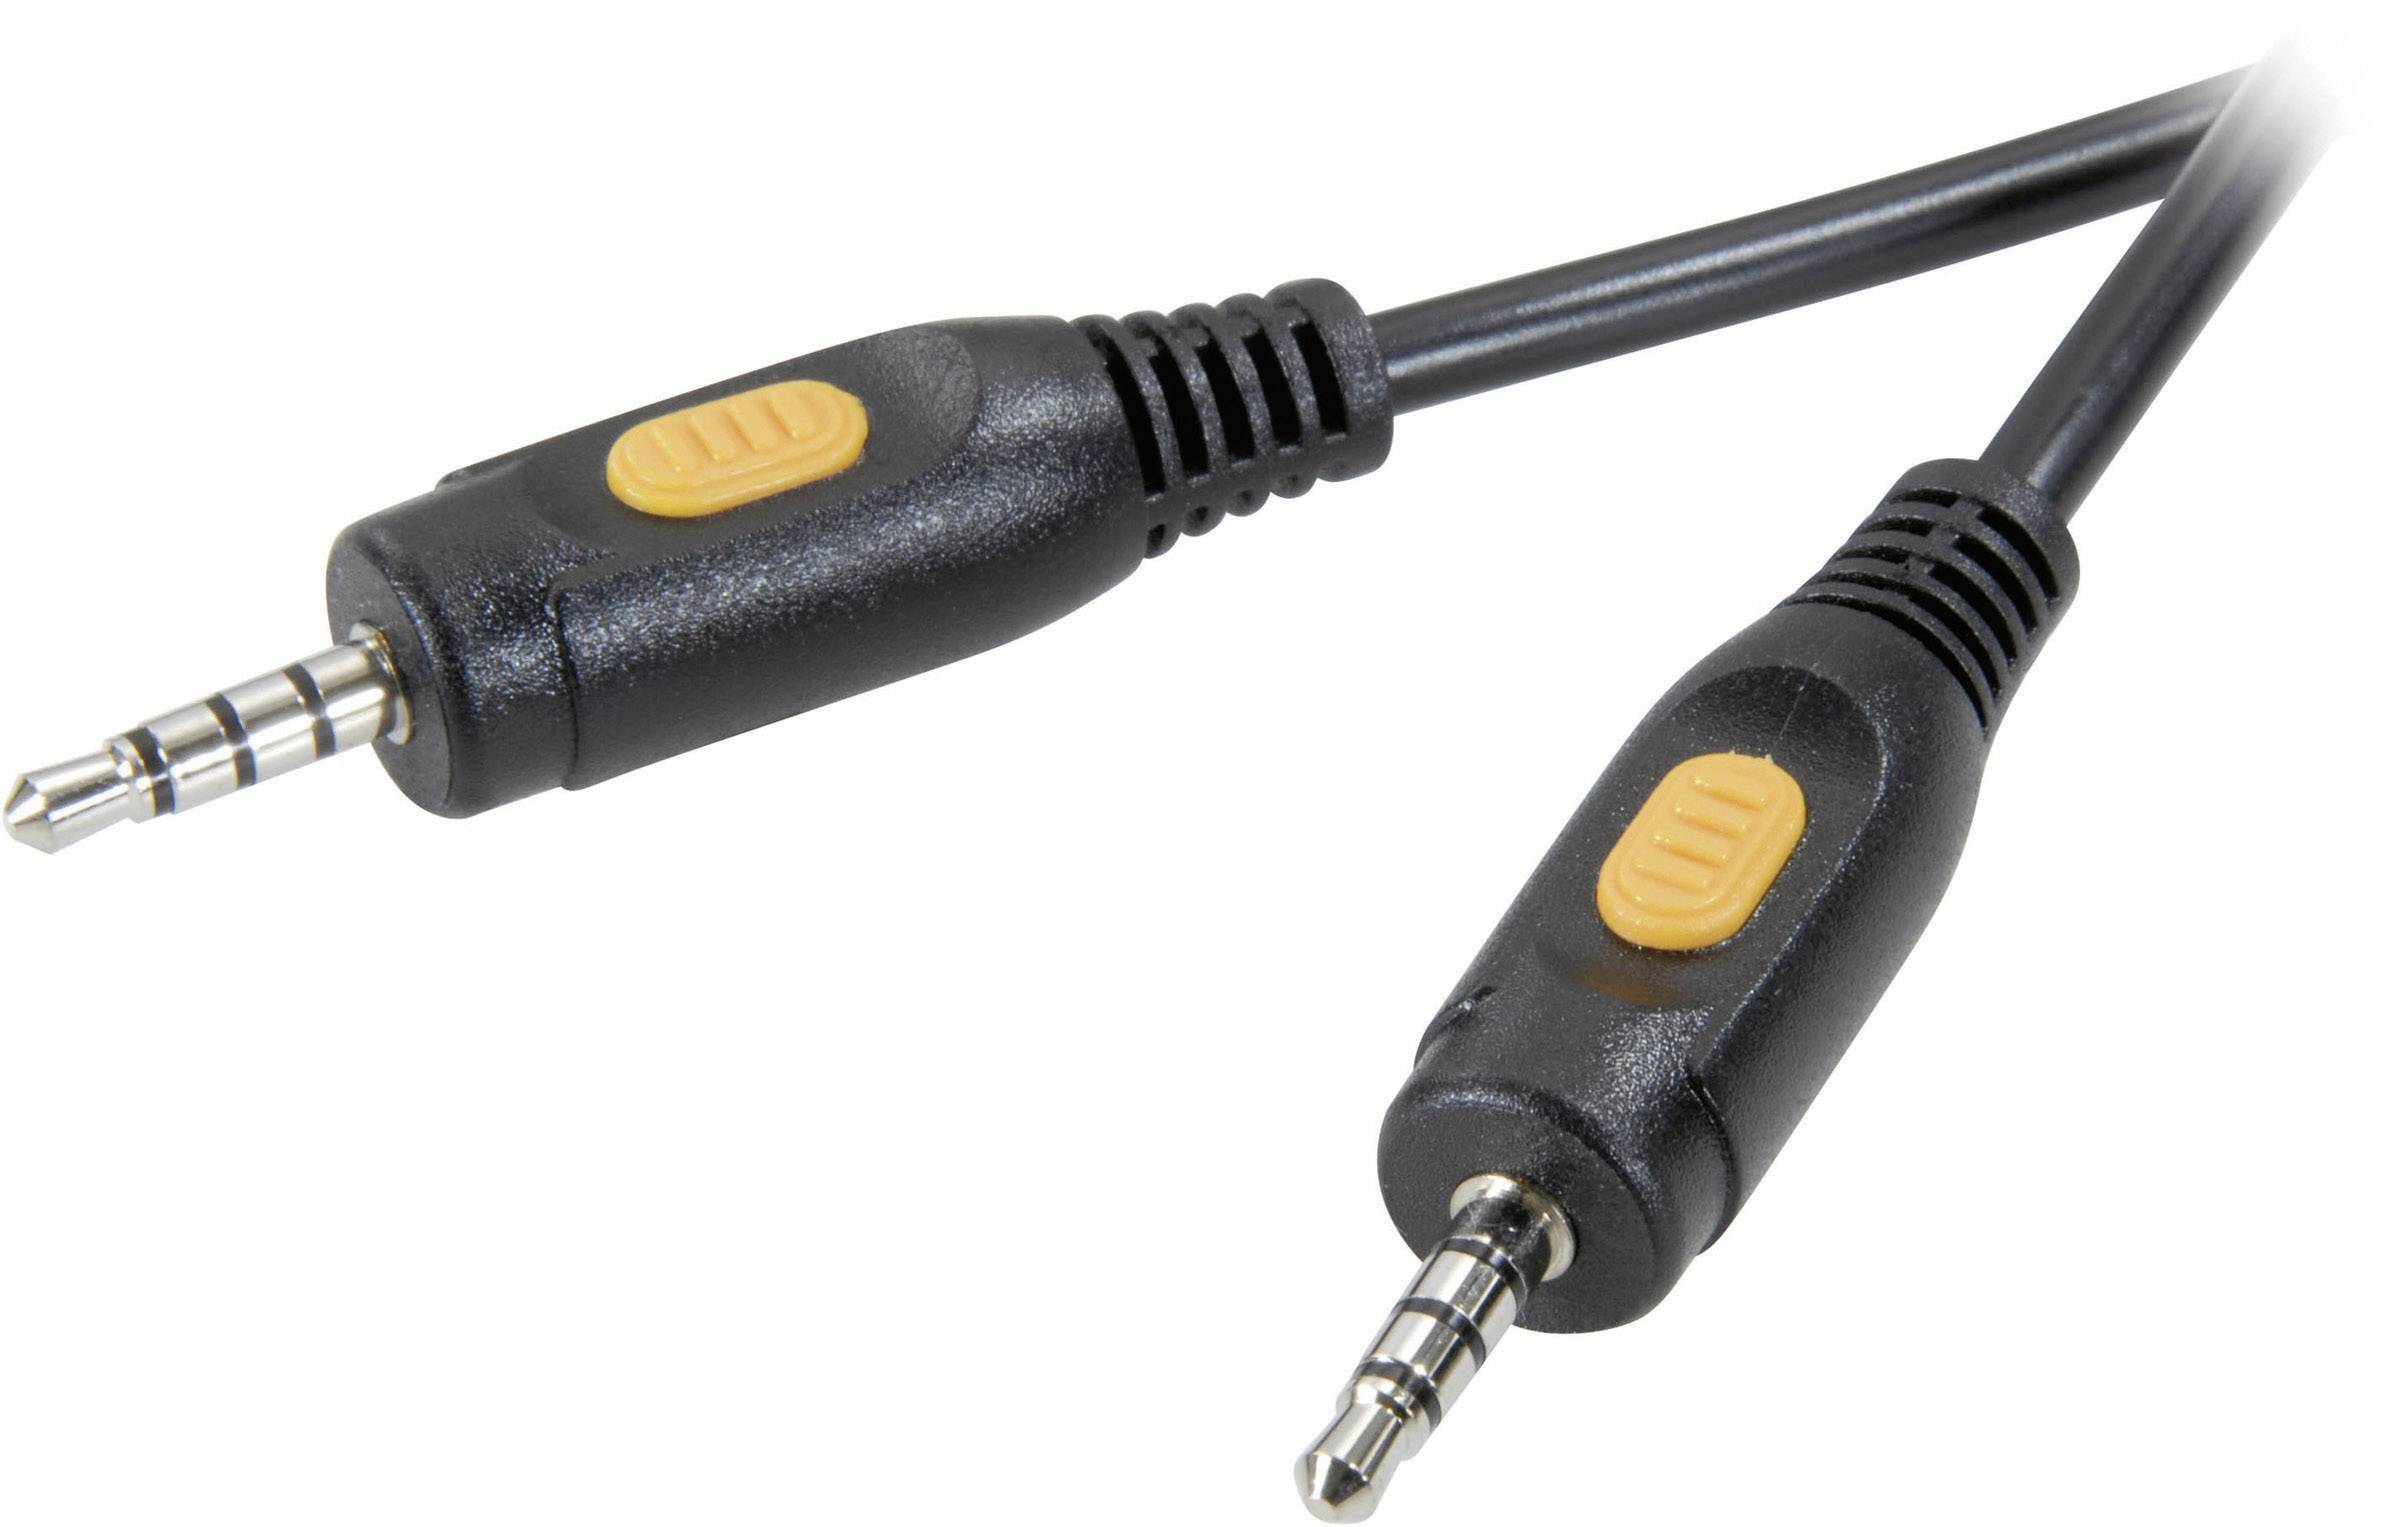
\includegraphics[width=0.6\textwidth]{jack}
\caption{The usual audio jack connector}
\label{fig:jack}
\end{figure}

\section{Environment}
The application consists of a desktop application developed in Python, some additional support scripts developed in Matlab to test the accuracy of the results. For testing purposes, an application called Audacity. As for the graphical user interface, it was chosen a simple approach using Tkinter
.
\subsection{File encoding formats}
The idea behind this method works for any audio format as long as new frequencies can be artificially injected into them. In the initial stages of prototyping of this project, several audio encoding formats were taken into consideration for this implementation: WAV, MP3, or FLAC. WAV being a raw encoding method, was chosen in the end as it provided a faster and easier way of modifying the sound. The major drawback of this choice would be the large size of files which result after this type of encoding
\subsubsection{WAV format}
Due to the simplicity of this format and its representation, WAV was chosen to be the type of the carrier sound for the messages encoded using the method which will be described further.
The WAV format, also known as WAVE(fig \ref{fig:wave}), was developed by Microsoft and, and it represented the standard for storing audio data on PCs. It is the leading way of storing on windows data in raw format and typically uncompressed audio files. As a result of this is the rather large size of files stored this way.

This type of format stores chunked data, a file consisting of several different sized chunks. Each chunk has a fixed sized header which describes the properties and the format of the data stored in the corresponding chunk such as the number of channels, byte rate or sample rate. The rest of the chunk represent actual information regarding the amplitude of the stored samples. This allows for an easy way of "inserting" artificial noise inside a sound file on a particular channel as long as the previous properties are respected.

\begin{figure}[h]
\centering
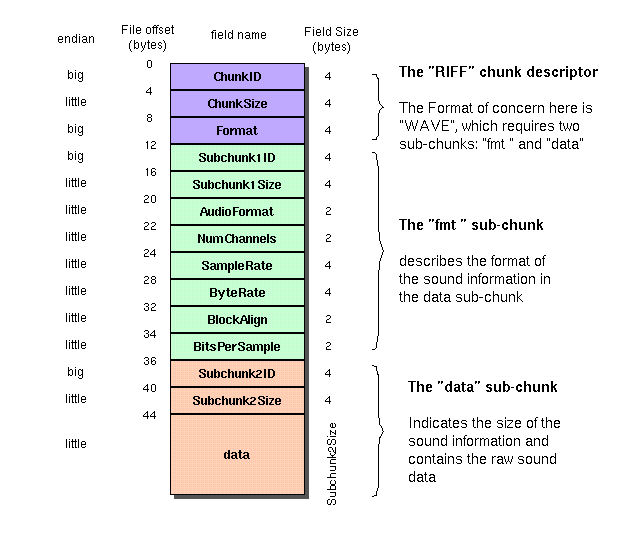
\includegraphics[width=1\textwidth]{wave}
\caption{WAV format}
\label{fig:wave}
\end{figure}

\subsection{Python programming language}

Python is an interpreted, high-level, general-purpose programming language. Created by Guido van Rossum and first released in 1991, Python has a design philosophy that emphasizes code readability, notably using significant whitespace. It provides constructs that enable explicit programming on both small and large scales. Van Rossum led the language community until July 2018.
Python is dynamically typed and garbage-collected. It supports multiple programming paradigms, including procedural, object-oriented, and functional programming. Python features a comprehensive standard library and is referred to as "batteries included"[ref here].

Python has always been the chosen language for prototypes and usually data processing algorithms as it provides a fast way of manipulating data, and provides a surprisingly good integration of Matlab methods and fast arithmetical computing provided by the instrumental library called Numpy.

Another reason for choosing Python as a base coding environment for this thesis is the ability to write code procedurally, a middle point between object-oriented programming and functional programming. However, this was more of an editor choice rather than provide real advantages in this aspect compared with other languages.
\subsection{Tkinter UI development in Python}
The Tkinter module ("Tk interface") is the standard Python interface to the Tk GUI toolkit from Scriptics (formerly developed by Sun Labs).
Both Tk and Tkinter are available on most Unix platforms, as well as on Windows and Macintosh systems. Starting with the 8.0 release, Tk offers a natural look and feel on all platforms.

Tkinter consists of a number of modules. The Tk interface is provided by a binary extension module named \_tkinter. This module contains the low-level interface to Tk, and should never be used directly by application programmers. It is usually a shared library (or DLL), but might in some cases be statically linked with the Python interpreter.

The structure of a UI designed using Tkinter has an arborescent nature.

\begin{figure}[h!]
\centering
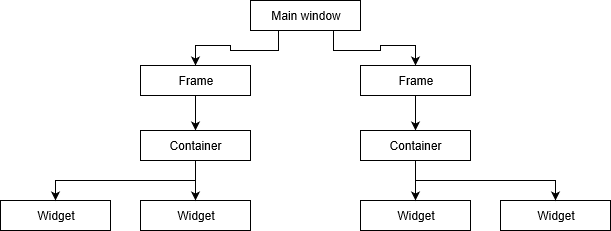
\includegraphics[width=1\textwidth]{tkinter}
\caption{Tkinter}
\label{fig:tkinter}
\end{figure}

\subsection{Matlab and matplotlib integration in Python}
Matplotlib is a Python 2D plotting library which produces publication quality figures in a variety of hardcopy formats and interactive environments across platforms. Matplotlib can be used in Python scripts, the Python and IPython shells, the Jupyter notebook, web application servers, and four graphical user interface toolkits.

Matplotlib tries to make easy things easy and hard things possible. You can generate plots, histograms, power spectra, bar charts, error charts, scatterplots, or many more other types of plots, with just a few lines of code. For examples, see the sample plots and thumbnail gallery.
For simple plotting, the pyplot module provides a MATLAB-like interface, particularly when combined with IPython. For the power user, you have full control of line styles, font properties, axes properties, via an object-oriented interface or via a set of functions familiar to MATLAB users.


\subsection{Numpy}
NumPy is the fundamental package for scientific computing with Python. It contains, among other things:
\begin{itemize}
  \item a powerful N-dimensional array object
  \item sophisticated (broadcasting) functions
  \item tools for integrating C/C++ and Fortran code
  \item useful linear algebra, Fourier transform, and random number capabilities
\end{itemize}
Besides its obvious scientific uses, NumPy can also be used as an efficient multi-dimensional container of generic data. Arbitrary data-types can be defined. This allows NumPy to seamlessly and speedily integrate with a wide variety of databases.

\section{Proposed method and personal contributions}
\subsection{Data representation}
Either talking about messages, images, or sounds, each of these can be represented using binary notation. In our case a sequence of letters can be uniquely described by another sequence of bytes; usually, such representations being ASCII or UTF-8, where characters are associated a number directly in a certain range of total possibilities. Each of these numbers can be subsequently represented in base 2, binary representation where a 0 can represent something an 1 something else. This creates a way of representing any complex message as a sequence of ones and zeroes.

What if we could somehow translate these ones and zeroes in audio data, and by this transforming any message into sound. This approach is found in the implementation of LSB techniques, where each bit from a message is translated directly to one bit in the hidden message. 

The way proposed to encode a message in this project further improves this idea, by creating fixed sized groups of bits from a message, each group representing a discrete number in base 10. By having this series of numbers, they can be uniformly associated with a certain frequency value from a predefined domain, preferably at e edge of human hearing.
(fig \ref{fig:data_representation})

\begin{figure}[h]
\centering
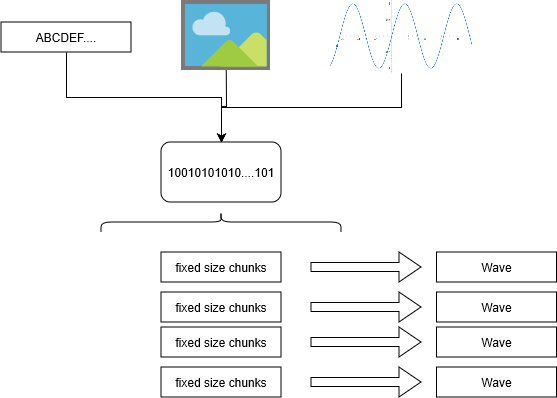
\includegraphics[width=1\textwidth]{data_repres}
\caption{Proposed data representation}
\label{fig:data_representation}
\end{figure}


\subsection{Noise generation}

After having translated the message into a series of frequencies, the next step is to generate sound corresponding to those frequencies in a way compatible with the chosen format of the carrier sound file. In our case WAV being a raw encoding format, this procedure reduces in generating the samples of a sound of that frequency without having to take care of the compression aspect of the digital sound data.

\begin{center}
\begin{math}
y(t) = A sin(2\pi f t + \varphi ) = A sin(\omega t + \varphi )
\end{math}
\end{center}

where:
\begin{itemize}

\item A, amplitude, the peak deviation of the function from zero.
\item f, ordinary frequency, the number of oscillations (cycles) that occur each second of time.
\item 
\begin{math} \omega = 2 \pi f \end{math}, angular frequency, the rate of change of the function argument in units of radians per second 
\item
\begin{math} \varphi \end{math}
, phase, specifies (in radians) where in its cycle the oscillation is at t = 0.
\end{itemize}

Using this equation, we can generate a sine wave for each frequency that we have obtained. The amplitude of the noise can be variable.

The human ear can recognize single sine waves as sounding clear because sine waves are representations of a single frequency with no harmonics. 
To the human ear, a sound that is made of more than one sine wave has perceptible harmonics; addition of different sine waves results in a different waveform and thus changes the timbre of the sound. Presence of higher harmonics in addition to the fundamental causes variation in the timbre, which is the reason why the same musical note (the same frequency) played on different instruments sounds different

\begin{figure}[h]
\centering
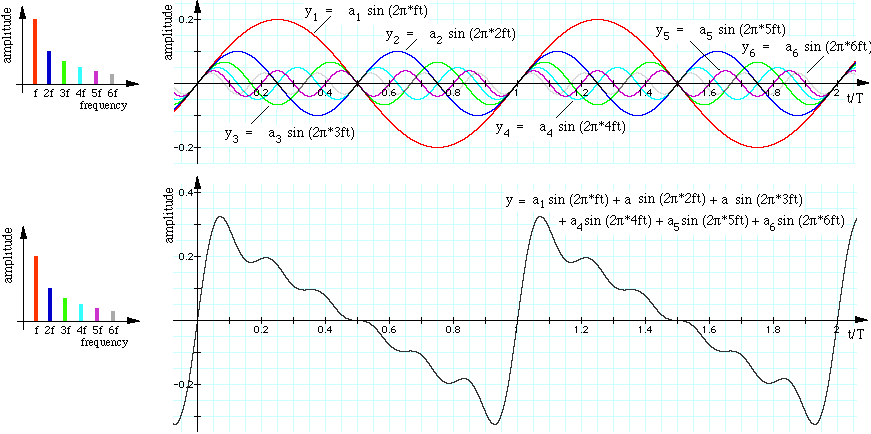
\includegraphics[width=1\textwidth]{combination}
\caption{Noise generation method}
\label{fig:noise_generation}
\end{figure}


\subsection{Noise combination with the original sound}
The noise is generated such that to be aligned with the original sound, meaning having the same sample rate. This ensures that the 2 waves can be combined by adding them, the result is a new wave with samples having the amplitude equal to the sum of the amplitudes corresponding to the samples at the target time frame. This needs to be clamped such that each frame to have the amplitude in the interval [-1, 1], resulting in some minor reconstruction errors for sounds that contain high amplitude samples. 

\begin{center}
\begin{math}
A(So) = ceva 
\end{math}
\end{center}


\subsection{The secret key}
This method can be considered to work similarly as a symmetric cipher. Both the sender and the recipient need to know certain critical information to be able to code and decode the message accurately. These parameters should be unable to be deduced just by looking at the sound in question.


After all these steps, the stego message is ready to be delivered.
\subsection{Reconstruction of the message}  
At the recipients' side, the message is reconstructed by repeated Fourier analysis over the sound. The sound is traversed using a window of the size specified in the key and transformed into the frequency domain. Due to transmission errors, the frequency searched might not have the correct value. However, here intervenes yet another problem. As seen in (fig \ref{fig:reconstruction}), the ideal case would be where target frequencies would be easily distinguishable and precise. Unfortunately, this rarely happens, due to transmission loss, approximations during computations or wave interferences the actual result of a Fourier transform would be something closer to (fig \ref{fig:approximation}). Here instead of 3 "peaks" corresponding to each target frequency, we have at least 5, if we consider 40 dB as detection threshold (the lower threshold, the more possible "peaks"). Even 5 peaks raise a significant problem as neither of them matches the original, intended, frequencies used for encoding. As one might notice, this might present a severe challenge for someone trying to break this method without knowing the secret key. Here the algorithm shines. Using the frequency granularity, the original frequency range used for encoding, and the length of the alphabet the position of the hidden information in the frequency domain can be deduced. After that, by taking into consideration the amplitudes of the peaks, the value of the initial frequency can be approximated using the nearest neighbor algorithm as the target frequency alphabet is known. 


\begin{figure}[h]
\centering
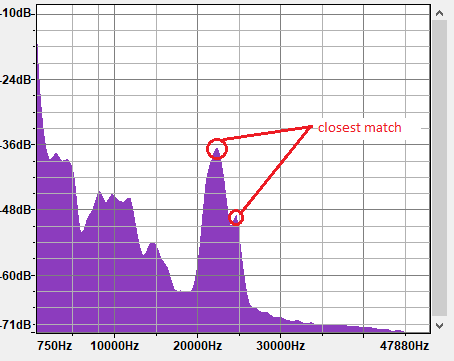
\includegraphics[width=1\textwidth]{reconstruction}
\caption{Reconstruction}
\label{fig:reconstruction}
\end{figure}

\begin{figure}[h!]
  \centering
  \begin{subfigure}[b]{0.9\linewidth}
    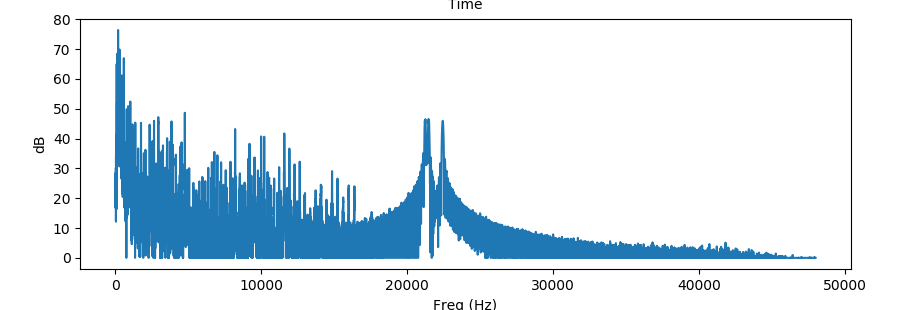
\includegraphics[width=\linewidth]{target_original}
    \caption{Oringial}
    \label{fig:original}
  \end{subfigure}
  \begin{subfigure}[b]{0.9\linewidth}
    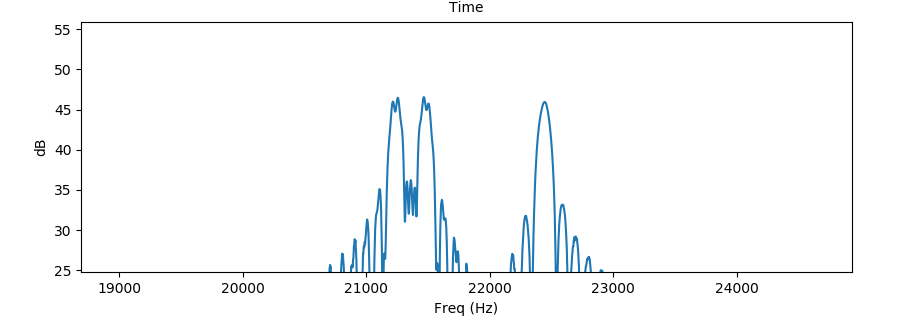
\includegraphics[width=\linewidth]{target_zoom}
    \caption{Zoomed}
    \label{fig:zoom}
  \end{subfigure}
  \begin{subfigure}[b]{0.9\linewidth}
    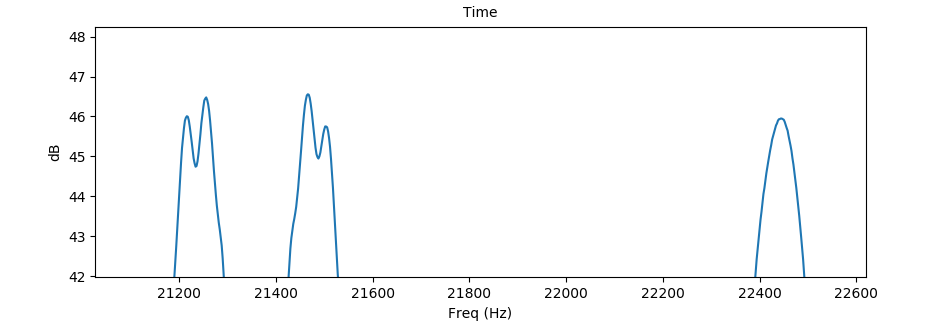
\includegraphics[width=\linewidth]{target__extra_zoom}
    \caption{Extra Zoomed}
    \label{fig:ezoom}
  \end{subfigure}
  \caption{Hillclimbing}
  \label{fig:approximation}
\end{figure}


\section{Steganalysis}
Due to the nature of the encoded frequencies spanning over several samples, decoding the message without knowing the secret key proves to be rather challenging. Apart from the other existing techniques like LSB where data is spread over each sample, using the frequency encoding, a chunk of data can cover several samples. Without the information regarding where certain frequencies are located, an FFT analysis can only confirm that those frequencies exist inside the stego-object.

Supposing the length of an encoded wave is known, meaning the key is partially compromised, it still requires to be able to pinpoint where in the sound was encoded the message. Using the Fast Fourier Transform one can confirm that a particular sound is composed of what frequencies but is unable to tell exactly which part of it contains them. 

As seen above, this method proves to be robust and can handle several degrees of data compromising before someone being able to break it without bruteforcing all the possible alternatives.


\section{Limitations}
The method presented above even having significant strong aspects, it suffers from some drawbacks caused by the use of these high frequencies. Most of them are regarding hardware issues, but there are also some limitations of software nature.

\subsection{Hardware limitations}
Since humans can't hear sounds having frequencies above a certain threshold,  usually somewhere around 21 kHz, companies that produce sound equipment(headphones, microphones) don't spend energy and time in developing systems that can handle frequencies above that limit. Only a few numbers of producers make such devices available, that could go as high as 40 kHz and cost about a fortune.

When the transmission environment of sounds that have been altered with this method is the air outside laboratory conditions, there can appear massive disruptions that can be recorded by the receiver. Even if techniques that minimize the interferences would be applied on the receivers end, such as low pass or high pass filters to diminish or augment the amplitude of specific frequencies, for better decoding, the message could present heavy losses.

Because of these limitations, the method of sending the stegofile from one place to another should happen only digitally, or analogically.

To test this method sounds where transmitted from one computer to another directly between sound cards using a Jack-Jack connection between them. One sound card played the role of the emitter and one of the receiver. This experiment simulates the behavior of sound transmission under absolutely ideal conditions, no interferences, and the loss being minimum during transmission. Soundcards are usually able to create continuous signals up to 48 kHz, so this environment presented more liberty when it came to the range of frequencies that could be used.




\begin{figure}[h!]
  \centering
  \begin{subfigure}[b]{0.4\linewidth}
    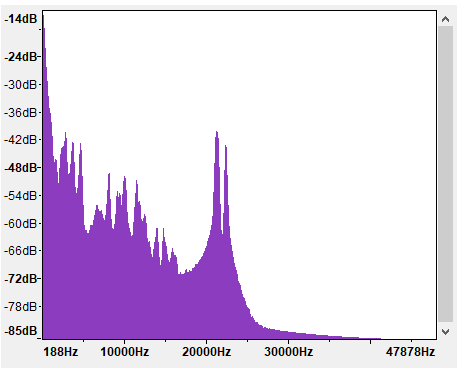
\includegraphics[width=\linewidth]{before_trans}
    \caption{Oringial}
    \label{fig:before_trans}
  \end{subfigure}
  \begin{subfigure}[b]{0.4\linewidth}
    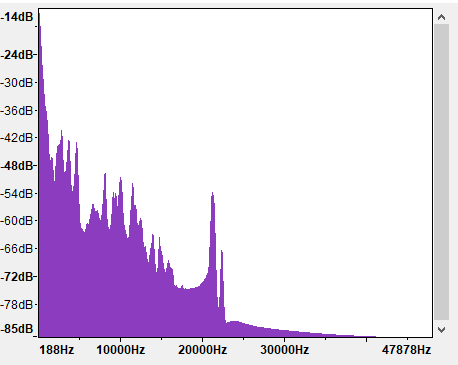
\includegraphics[width=\linewidth]{after_trans}
    \caption{Zoomed}
    \label{fig:after_trans}
  \end{subfigure}
  \caption{Data loss}
  \label{fig:data_loss}
\end{figure}


\subsection{Software limitations}

There exists a limit to the amount of raw data that can be hidden using this method. This threshold is heavily influenced by the granularity of which we want to encode the message. In this project, I defined 3 kinds of granularity which influence the algorithm: chunk granularity and frequency granularity.

\subsubsection{Frequency granularity}
This type mainly refers to the distance between the frequency values used in the encoding and is directly proportional to the size of the interval of frequencies used. Having an array of used frequencies, those should be equidistant in value to each other (delta F). This parameter is important because should it be too small, the decoding gets to imprecise and start to fail, but the larger it gets, the larger the range of frequencies will be. On low frequency, granularity represents how far are the frequencies used from one another.

\subsubsection{Chunk granularity}
This type of granularity refers to the amount of data that could be described by a single frequency. Let us suppose our alphabet contains 8 symbols: A B C D E F G H. We could encode each element using one frequency, but this comes with some drawbacks. In the case of a large alphabet, the range of frequencies also increases, supposing we use the same frequency granularity. What could be done instead is group 2 or more alphabet elements and characterize each unique group by a frequency. This drastically improves the amount of data that could be encoded in a certain sized, but it increases the number of frequencies used in the process from n to comb(n,k).

\subsubsection{Noise granularity}
To further control the amount of hidden data, this last kind of granularity was introduced. It represents how far, in seconds, are waves distanced from one another. This is also the size in seconds of the scan window used in the decoding process. Being close it increases the amount of data able to be hidden, but it increases the risk that the Fourier analysis to miss frequencies.


\begin{table}
\centering
\begin{tabular}{|c|c|c|c|c|c|} 
\hline
\begin{tabular}[c]{@{}c@{}}Sound\\Duration\\(sec)\end{tabular} & \begin{tabular}[c]{@{}c@{}}Noise\\Granularity\\(sec)\end{tabular} & \begin{tabular}[c]{@{}c@{}}Noise\\Lenght\\(sec)\end{tabular} & \begin{tabular}[c]{@{}c@{}}Chunk\\Granularity\\(bit)\end{tabular} & \begin{tabular}[c]{@{}c@{}}Frequency\\Granularity\end{tabular} & \begin{tabular}[c]{@{}c@{}}Max~\\Message\\Length\\(kb)\end{tabular}  \\ 
\hline
1                                                              & 0.01                                                              & 0.1                                                          & 8                                                                 & 256                                                            & ~0.8                                                                 \\ 
\hline
2                                                              & 0.02                                                              & 0.1                                                          & 9                                                                 & 512                                                            & 1.5                                                                  \\ 
\hline
5                                                              & 0.03                                                              & 0.1                                                          & 10                                                                & 1024                                                           & 3.8                                                                  \\ 
\hline
5                                                              & 0.01                                                              & 0.2                                                          & 9                                                                 & 512                                                            & 3.7                                                                  \\ 
\hline
100                                                            & 0.001                                                             & 0.001                                                        & 12                                                                & 4096                                                           & 600                                                                  \\ 
\hline
10                                                             & 0.01                                                              & 0.01                                                         & 8                                                                 & 256                                                            & 30                                                                   \\ 
\hline
10                                                             & 0.01                                                              & 0.01                                                         & 9                                                                 & 512                                                            & 40                                                                   \\ 
\hline
10                                                             & 0.01                                                              & 0.01                                                         & 10                                                                & 1024                                                           & 45                                                                   \\
\hline
\end{tabular}
\caption{Data quantity limitation}
\label{tab:table}
\end{table}


\chapter{Comparison with existent methods}

\section{Other techniques}
The number of other methods used for hiding messages has seen a continuous increase over the years. I will present only some of the most frequently used in audio frequency, but this list is far from being exhaustive. Each of these methods comes with its advantages or disadvantages which will be discussed later.
\subsection{Structural methods}
These kinds of methods rely on hiding data by changing or abusing the metadata of the carrier file, such as headers. This techniques are commonly seen in image steganography as most file format headers contain information regarding the size of the raw data of the file, especially those that contain raw uncompressed data. One such approach could be writing the message after the total size specified in the header. Although these methods seem efficient, based on what software is used to render the image, if certain file integrity checks are performed, the stego-file could become unusable by the user, ending in raising suspicions over the file.

\subsection{LSB \emph{(least significant bit}) method}
Least significant bit  (LSB)  coding is the simplest way to embed information in a digital audio file.  By substituting the least significant bit of each sampling point with a binary message, LSB 
coding allows for a large amount of data to be encoded. Extraction process retrieves the watermark by reading the value of these bits from the stego-object.
The standard method usually encodes bits one by one, thus resulting in a most accurate to the unmodified version of the original sound. This method can be applied over each sample or each frame of the sound. The more bits used from the message and hidden in a single frame, the higher the quantity of data that can be hidden, trading off the quality of the carrier sound which could lead to suspicions, and as I stated above the method has to be extremely subtle as an experienced steganalyst will firstly check the LSB method by isolating the last bits and recovering the message.

\begin{figure}[h]
\centering
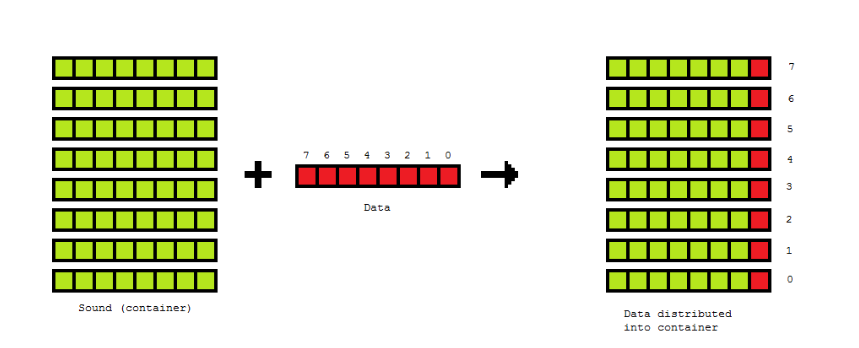
\includegraphics[width=1\textwidth]{lsb}
\caption{LSB}
\label{fig:LSB}
\end{figure}

\subsection{Phase coding}
Humans usually cant discern phase changes in the phase of sounds. That is why a cosine wave of x Hz is heard the same as a sine. The basic idea is to split the original audio stream or cover file(C) into blocks and embed the whole message data sequence into the phase spectrum of the first block. One drawback of the phase coding method is a considerably low payload because only the first block is used for secret message (M) embedding.
\begin{figure}[h]
\centering
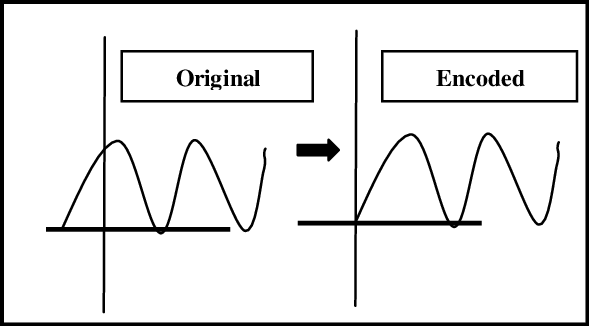
\includegraphics[width=1\textwidth]{phase}
\caption{Phase coding}
\label{fig:phase}
\end{figure}

\section{Advantages/disadvantages}
These methods share common aspects such as each one encoding raw data by splitting the message into bits and then encoding the one by one or in chunks. LSB suffers from the lack of customization, the method being rather simple, and thus making it the first idea which comes in mind when it comes to decoding a potential stego-object.

Phase coding relies upon the discrete Fourier transform, which compared to the fast Fourier transform is much slower, making it less efficient when it comes to large files compared to the high-frequency encoding.

\chapter{Further improvements and real-life examples}
\section{Further improvements}
This method currently encodes raw data. This lowers the amount of data that could be hidden in a WAV file. Such as MP3 files use data compression, similar methods could be implemented to compress the message to make it more compact, resulting in more data hidden.
To make the transmission even more unbreakable, a layer of encryption could be added above the massage before encoding.

\section{The dolphin attack}
Digital assistants, like Google's Assistant, Apple's Siri, and Amazon's Alexa, are becoming more and more popular as the world embraces this new Artificial Intelligence technology, built to make our lives easier. The big companies are competing for who has the most effective product, and one way to do this is to make the digital assistants more personalized and tailored to individual users. To achieve this, however, a great deal of personal information needs to be shared with the device, and this can be a goldmine for cyber-criminals.
Researchers claim to have found a way to hijack the voice-controlled assistants, by using ultrasonic audio commands that dolphins can hear, but humans cannot. On most smartphones, the digital assistant is set up to listen for a "wake word". For Google, the assistant takes orders once a person says, "OK Google", while Apple's assistant responds to "Hey Siri" and Amazon's to "Alexa".
Chinese researchers from Zhejiang University decided to create a program that could translate a standard human voice command and broadcast it in ultrasonic frequencies (over 20 kHz). These frequencies are too high for humans to hear, but they wanted to see if they were still audible to smartphones. To play these frequencies, the program needed basic equipment, such as a smartphone, amplifier, ultrasonic transducer and battery, costing a mere 3 dollars for the parts.

\begin{figure}[h!]
  \centering
  \begin{subfigure}[b]{0.4\linewidth}
    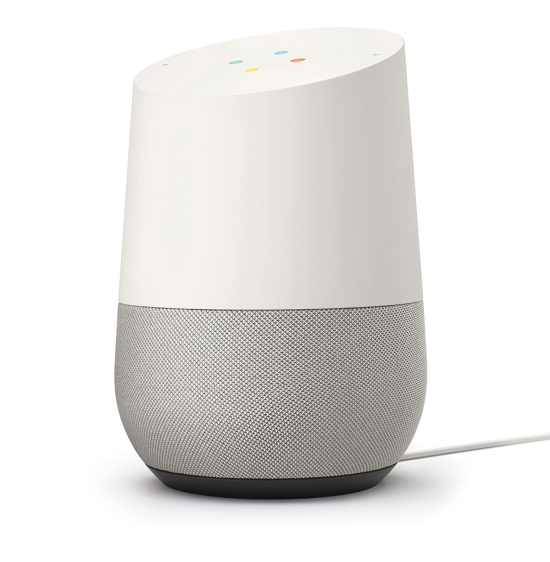
\includegraphics[width=\linewidth]{google_home}
    \caption{Google Home}
    \label{fig:g_home}
  \end{subfigure}
  \begin{subfigure}[b]{0.4\linewidth}
    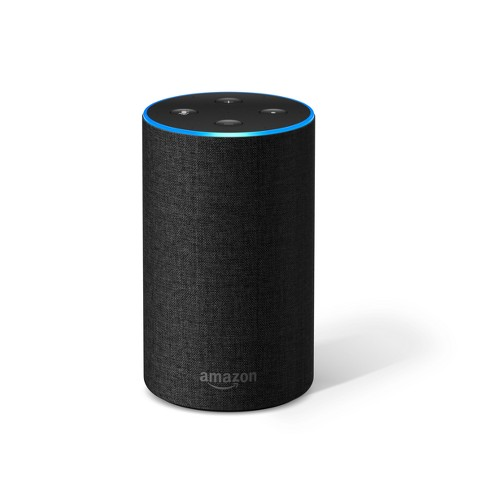
\includegraphics[width=\linewidth]{alexa}
    \caption{Amazon Alexa}
    \label{fig:alexa}
  \end{subfigure}
  \caption{Examples of assistants}
  \label{fig:assistants}
\end{figure}


\listoffigures
 
\listoftables



\begin{thebibliography}{6}
\bibitem{note1}
Katzenbeisser, S., Petitcolas, F.A.P.: Information Hiding: Techniques for steganography 
and digital watermarking. Artech House, Boston (1999) 
\bibitem{note2}
Mahendra Kumar Pandey, Girish Parmar, and Sanjay Patsariya:An Effective Way to Hide the Secret Audio File Using 
High Frequency Manipulation (2011)
\bibitem{note3}
Ahmed Hussain Ali,Mohd Rosmadi Mokhtar and LoayEdwar George: A Review on Audio Steganography Techniques (2015)
\bibitem{note4}
Pahati, OJ (2001-11-29). "Confounding Carnivore: How to Protect Your Online Privacy". AlterNet. Archived from the original on 2007-07-16. Retrieved 2008-09-02.
\bibitem{note5}
Candes, E. J., Wakin, M. B. (2008). An Introduction To Compressive Sampling. IEEE Signal Processing Magazine, 25(2), 21-30. doi:10.1109/MSP.2007.914731
\bibitem{note6}
Marler, Peter (2004). Nature's Music: The Science of Birdsong. Academic Press Inc. p. 207. ISBN 978-0124730700
\bibitem{note7}
Stéphan Blatrix, www.neuroreille.com, 1999
\end{thebibliography}


\end{document}